% Created 2019-12-29 Sun 20:03
% Intended LaTeX compiler: pdflatex
\documentclass[a4paper, 11pt]{extarticle}
             \usepackage[utf8]{inputenc}
\usepackage[left=2cm, right=2cm, bottom=2.5cm, top=2.5cm]{geometry}
% Paquetes de matemáticas
\usepackage{amsmath, amsfonts, amssymb, commath}
\usepackage{tikz}
\usepackage{tikz-cd}
\newcommand{\tikzcircle}[2][red,fill=red]{\tikz[baseline=-0.5ex]\draw[#1,radius=#2] (0,0) circle ;}%
% Ajustes de idioma, gráficos, etc
\usepackage{adjustbox}
\usepackage{float}
\usepackage{hyperref}
\usepackage{graphicx}
\usepackage{gensymb}
\usepackage[spanish, english]{babel}
\usepackage{tikz}
\usepackage{multicol}
\usepackage{listings}
\usepackage{enumitem}
\setlist{nolistsep}
\usepackage{booktabs}
\usepackage{xcolor}
\usepackage{wrapfig}
%Fuentes.
% Alegreya tiene este toque antiguo con serifa, y la tipografía de las ecuaciones es también interesante.
% Gillius no tiene serifa, y también es equilibrada.
\usepackage[T1]{fontenc}
%\usepackage[default]{gillius}
\usepackage{newpxtext, newpxmath}
% Paquete para añadir Creative Commons al final del documento
\usepackage[
type={CC},
modifier={by-nc-nd},
version={3.0},
]{doclicense}
% Propiedades de párrafo
\setlength{\parindent}{0em}
\setlength{\parskip}{1.1em}
\renewcommand{\baselinestretch}{1.05}
\setlength\itemsep{0em}
% Definición de comandos. Muchos de ellos han surgido para Geometría, aunque se
% irá actualizando la lista. POSIBLEMENTE LO INTRODUZCA COMO COMANDOS DE ORG
\newcommand{\m}{\text{medio}}
\newcommand{\iso}{\text{Isom}}
% Para incluir mathcal en las ecuaciones. El /mathcal para Alegreya es el viejo
% y floritural estilo que odio.
\usepackage{calrsfs}
\DeclareMathAlphabet{\pazocal}{OMS}{zplm}{m}{n}
% Definición de colores agradables a la vista
\definecolor{azul}{HTML}{107896}
\definecolor{naranja}{HTML}{C2571A}
\definecolor{rojo}{HTML}{9A2617}
\definecolor{amarillo}{HTML}{BCA136}
\definecolor{verde}{HTML}{829356}
\definecolor{gris}{HTML}{909090}
\definecolor{rosa}{HTML}{F9A7B0}
\definecolor{amarillochillon}{HTML}{FBB117}
% Definición de comandos para teoremas, etc. El comando también incluye
% como argumento un texto, del estilo Teorema 3.5
\newcommand{\axioma}[1]{\textcolor{naranja}{\textbf{Axioma #1}}}
\newcommand{\tma}[1]{\textcolor{rojo}{\textbf{Teorema #1}}}
\newcommand{\propo}[1]{\textcolor{rojo}{\textbf{Proposición #1}}}
\newcommand{\defi}[1]{\textcolor{azul}{\textbf{Definición #1}}}
\newcommand{\obs}[1]{\textcolor{verde}{\textbf{Observación #1}}}
\newcommand{\ejem}[1]{\textcolor{verde}{\textbf{Ejemplo #1}}}
\newcommand{\ej}[1]{\textcolor{amarillo}{\textbf{Ejercicio #1}}}
\newcommand{\lema}[1]{\textcolor{rosa}{\textbf{Lema #1}}}
\newcommand{\cor}[1]{\textcolor{rosa}{\textbf{Corolario #1}}}
% La demostración es igual pero va con una letra más pequeña y en gris.
\newcommand{\dem}[1]{\textcolor{gris}{\small{Demostración. #1}}}
% Esto pone un triangulito de peligro para cuando algo es importante.
\newcommand{\importante}{\tikzcircle[amarillo, fill=amarillo]{4pt}\,}
% Para usar columnas emplea este trozo de código
% \begin{multicols*}{2}
% [\section{Axiomas para la geometría euclidiana plana}]
% 	\axioma{P1} Si tenemos el conjunto $\P$, denominado \textbf{plano}, y la aplicación $d:\P \times \P \rightarrow \R$ llamada \textbf{distancia}, entonces$(\P, d)$ es un espacio métrico.

\defi{2.2} Una \textbf{recta} $r \subset \P$ satisface
\begin{itemizex}
	\item $r$ contiene al menos dos puntos.
	\item Para toda terna de puntos $A, B, C$, están alineados si están en $r$.
\end{itemizex}

\axioma{P2} $\P$ contiene al menos tres puntos no alineados; y por dos puntos distintos, $A$ y $B$ de $\P$ pasa una recta, $r_{AB}$.

\defi{2.6} / \tma{2.7} Dos rectas se cortan si sólo tienen un punto en común, y si no tienen ningún punto en común, entonces se denominan \textbf{paralelas}, y se denota por $a \parallel b$. Dos rectas, o se cortan o son paralelas.

\importante\axioma{P3} Para toda recta $r \subset \P$ existe una biyección $\gamma: r \rightarrow \R$ tal que $|\gamma(X) - \gamma(Y)| = |x - y| = d(X, Y) \;\; \forall \;\; X,Y \in r$ 

\obs{2.8} Si $A, B \in r$ son distintos, entonces existe un punto $M\in r: d(A,M) = d(M,B)$ que denotamos por $\m[A,B]$ y se llama \textbf{punto medio}. Asimismo sólo existe un punto $B \in r$ tal que $B = \m[A, M]$.

\obs{2.9} Si $r$ es una recta y $P \in r$, entonces $r$ se puede dividir en dos \textbf{semirrectas}, que son los conjuntos $\{X \in r \; | \; \gamma(X) > \gamma(P)\}$ y $\{X \in r \; | \; \gamma(X) < \gamma(P)\}$.

\axioma{P4} Para toda recta $r \subset \P$ hay dos subconjuntos $H^1$ y $H^2$, denominados \textbf{semiplanos} de $r$, que verifican:
\begin{itemizex}
	\item $H^1 \cup H^2 = \P-r$
	\item Si $X,Y \in H^i$ entonces $[X,Y] \subset H^i$
	\item Si $X \in H^1$ y $Y \in H^2$ entonces $[X,Y] \cap r \neq \emptyset$.
\end{itemizex}

\defi{2.15} Sean $P, Q, R$ no alineados, entonces el triángulo $\triangle\{P,Q,R\}$, o $\triangle PQR$ está formado por los segmentos $[P,Q]$, $[Q,R]$, $[P,R]$, llamados lados, y los vértices $P,Q, R$.

\tma{2.16 [Axioma de Pasch]a} Dado un triángulo $\triangle PQR$ y una recta $r$; si $r$ corta a $[P,Q]$, entonces o corta a $[P,R]$ o a $[Q, R]$.

\defi{2.17 = 1.5} Una \textbf{isometría} en $\P$ es una biyección $g: \P \rightarrow \P$ que cumple que $d(g(X), g(Y)) = d(X,Y) \;\;\forall\;\; X,Y \in \P$.

\tma{2.18} Si $A,B \in \P$ y $g \in \iso(\P)$ entonces $g([A,B]) = [g(A), g(B)]$ y $g(r_{AB}) = r_{g(A)g(B)}$ 

\axioma{P5} Si $A_1, A_2 \in \P$ y $B_1, B_2 \in \P$ son dos pares de puntos que cumplen $d(A_1,A_2) = d(B_1,B_2)$ entonces existe $g \in \iso(\P)$ tal que $g(A_i) = B_i$. Se dice que esos pares de puntos son \textbf{congruentes}.

\axioma{P6} Para toda recta $r$ existe una isometría $\sigma$ llamada \textbf{reflexión} tal que  
\begin{itemizex}
	\item $\sigma(X) = X\iff X \in r$
	\item $\sigma \circ \sigma = \text{Id}$
\end{itemizex}


\defi{2.23} / \tma{2.25} / \cor{2.30} Una recta $l$ es \textbf{ortogonal} a $r$ si para todo $S \in l$ y para todo par de puntos $A, B$ que cumple que $M = \m[A,B]$, de modo que $l \cap r = M$, entonces se da que $d(A,S) = d(S,B)$. Se denota $l \perp_M r$. En estas condiciones, $l = \{X \in \P \; | \; d(S,A) = d(S,B)\}$, se denomina \textbf{mediatriz} de $[A,B]$. 

\begin{figure}[H]
	\centering
	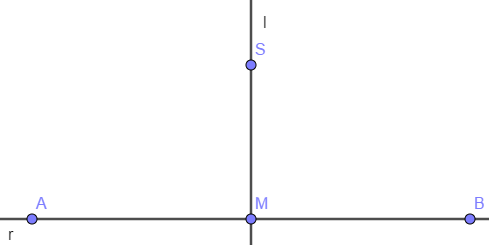
\includegraphics[width=7cm]{figuras/2-23.png}
	\vspace{-1em}
\end{figure}

\lema{2.21} Si $\sigma_r$ entonces, para todo $X$, $\m[X, \sigma_r(X)] \in r$.

\obs{2.24} Si $l \perp r$ y $g \in \iso(\P)$ entonces $g(l) \perp g(r)$.

\importante\tma{2.26} Si $l, r \subset \P$ cortan en $M$ y $\sigma_l, \sigma_r$ son dos reflexiones de $l$ y $r$, entonces se cumple que $l \perp_M r \iff r \perp_M l \iff \sigma_r(l) = l \iff \sigma_l(r) = r$.

\importante\tma{2.27 / 2.29} Para toda recta $r$ y todo punto $S \in \P - r$, existe una recta $l$ ortogonal a $r$, que pasa por $S$. Si $r$ es una recta, y $M \in r$, entonces existe $l$ tal que $l \perp_M r$.

\axioma{P7} Para toda recta $r$ y todo punto $P$ existe sólo una recta \textbf{paralela} a $r$ que pase por $P$.

\tma{2.31 / 2.33} Si $a \perp l$ y $b \perp l$ entonces $a \parallel b$. Sean $a \parallel b$. Entonces, para todo $A \in a$, la única recta $l \perp_A a$ también es ortogonal a $b$.

\tma{2.32} Las rectas parallelas forman una relación de equivalencia.
\begin{itemizex}
	\item Reflexividad: $a\parallel a$
	\item Simetría: $a \parallel b \rightarrow b \parallel a$
	\item Transitividad  $a \parallel b $ y  $b \parallel c \rightarrow a \parallel c$
\end{itemizex}

\ej{2.6} Sean $A,B \in r$, $A \neq B$. Para todo $t$, existe un único $P_t\in r$ que cumple $d(P_t,A) = \abs{t}$ y $d(P_t, B) = \abs{t-d(A,B)}$. En definitiva, la posición de $P_t$ está sólamente determinada por las distancias $d(A, P_t)$ y $d(P_t, B)$.
	 
	 
	 
	 
	 
	 
	 \end{multicols*}\pagebreak
% multicols* obliga a terminar una columna antes de empezar la siguiente.
\DeclareMathAlphabet{\pazocal}{OMS}{zplm}{m}{n}
\let\mathcal\pazocal
\usepackage{fancyhdr}
\pagestyle{fancy}
\lhead{Alex Martínez Ascensión}
\chead{}
\rhead{\today}
\date{}
\title{\Huge\vspace{-1em}Álgebra}
\hypersetup{
 pdfauthor={},
 pdftitle={\Huge\vspace{-1em}Álgebra},
 pdfkeywords={},
 pdfsubject={},
 pdfcreator={Emacs 26.2 (Org mode 9.2.5)}, 
 pdflang={English}}
\begin{document}

\maketitle
\vspace{-8em}

\section*{Anillos}
\label{sec:orgbe6d9a8}
\vspace{-1em}
\subsection*{Generalidades}
\label{sec:org15c74e1}
\vspace{-1em}
\defi{1.1 (Anillo)} Un \textbf{anillo} es una estructura \((A, +, \cdot)\) con las
propiedades: \vspace{-1em}
\begin{itemize}
\item \((A, +)\) es un grupo conmutativo
\item Asociatividad: \((xy)z = x(yz)\)
\item Distributividad: \((x + y)z = xz + yz \qquad x(y+z) = xy+xz\)
\end{itemize}
Se denota al elemento unitario de \((A, +)\) por \(0_A\) y al unitario de 
\((A, +, \cdot)\), si existe, por \(1_A\). \(A^* = A\\ \{ 0 \}\). \(0_A =
1_A \iff A = \{ 0 \}\).

\defi{1.6} Si \(1_A \in A\), entonces \(A\) es un \textbf{anillo unitario}. Una
\textbf{unidad} de \(A\) es un elemento \(x\) que tiene su inverso \(y\): \(xy=1\). El conjunto de unidades es \(U(A)\). El inverso, si existe, se puede denotar por \(x
^{-1}\) y \(x/y = xy ^{-1}\).

\defi{1.8} Un \textbf{cuerpo} es un anillo \(K\) tal que \(K^*\) es un grupo. O, un
anillo unitario con inverso.  

\defi{1.10} Un \textbf{divisor de cero} es un elemento \(x \in A^*\) tal que, para
algún \(y \in A^*\), \(xy = 0_A\). Un cuerpo nunca tiene divisores de cero:
\(x = x(yy ^{-1}) = (xy) y ^{-1} = 0 y ^{-1} = 0\)

\defi{1.11} Se denomina \textbf{dominio de integridad} a un anillo unitario sin divisores
de cero. El producto de dos anillos conmutativos \(C = A \times  B\) nunca es
un dominio de integridad, pues \((a, 0) \neq 1_A, (0, b) \neq 1_B\) y \((a, 0) \times (0, b) = (0, 0) = 0_C\).

A un dominio de integridad se le puede asociar un cuerpo mediante el \textbf{cuerpo de
fracciones de un dominio}. 
Dada la relación \((x,y) R (x', y') \iff xy' = x'y\), para el producto de dominios \(A \times  A^*\) 
entonces para la clase de equivalencia \([x,y]\), las operaciones \([x,y] +
[x', y'] = [xy' + y'x, yy'], [x,y]\cdot [x',y'] = [xx', yy']\) forman un
cuerpo, \(K\), con \(0_K = [0, 1]\), \(1_K = [1,1]\), y \([x,y] ^{-1} =
 [y, x]\).

\defi{1.14 (Ideal)} Un \textbf{ideal} es un subconjunto \(I \subset A\) tal que \vspace{-1em}
\begin{itemize}
\item \(I\) es subgrupo de \(A\)
\item \(\forall i \in I, a \in A, ia \in I\).
\end{itemize}
\(A, \{ 0 \}\) son los \textbf{ideales triviales}, y si \(I \neq A\), \(I\) es un  
\textbf{ideal propio}. Si \(1_A \in I\), \(I = A\): \(\forall a \in A\), \(a = a
\cdot 1\), y como \(1 \in I, a \in I\).

\defi{1.16} Dado un ideal \(I\) de \(A\), dada la relación \(xRy \iff x-y
\in I\), se forma el \textbf{anillo cociente} \(A/I\) con las clases de equivalencia
\([x] = x + I = \{ x + a \;|\; a \in I  \}\).
Las operaciones suma y producto definidas por \((x + I) + (y + I) = (x + y) +
I, \; (x + I)(y + I) = xy + I\), son inyectivas.

\defi{1.17 - 1.19} Sea \(A\) un anillo conmutativo y \(L\) un subconjunto de \(A\). El conjunto \(I\) de sumas finitas \(a_1x_1 + ... + a_lx_l,\; a_i \in A,
l_i \in L\) es un \textbf{ideal generado por \(L\)}. Además, \(I\) es el mínimo 
ideal que contiene a \(L\). Si \(L\) es finito, \(I\) es \textbf{finitamente generado}; y si \(L\) tiene
un solo elemento, es decir, \(I = Al\), el ideal es \textbf{principal}.

En los ideales se definen la (1) suma: \(I + J\) está dado por \(a_1, \cdots,
a_r, b_1, \cdots, b_s \in A, x_1, \cdots, x_r \in I, y_1, \cdots, y_s \in J,
a_1x_1 + \cdots + a_rx_r + b_1y_1 + \cdots + b_sy_s = x + y\); (2) producto: IJ
= \(x_1y_1 + \cdots + x_ry_r, x_1, \cdots, x_r \in I, y_1, \cdots, y_r \in J\), (3) intersección \(I \cap J\).

\defi{1.21} Un ideal es \textbf{maximal} si (1) \(A/I\) es un cuerpo y (2) \(I\) es
propio y ningún otro ideal propio lo contiene. \((1) \iff (2)\).
\textcolor{gray}{\footnotesize Si \( A/I  \) es
un cuerpo, luego contiene una unidad. Ninguna unidad \( i \) de \( A/I  \) puede estar
en \( I^* = I + i \) porque entonces \( I^* = A \)}.

\defi{1.22} Sean \(A\) unitario e \(I\) un ideal. Se dice que \(I\) es
\textbf{primo} si (1) \(A/I\) es un dominio de integridad y (2) \(I\) es propio, y
\(\forall x,y \in A\), si \(xy \in I\), \(x \in I\) o \(y \in I\). \((1) \iff (2)\).
\dem{ Si \( xy \in I  \), \( 0 + I = xy + I = (x+I)(y+I) \). Como \( A/I  \) es dominio, 
\( x+I = 0 + I \rightarrow x \in I \) o \( y+I = 0 + I \rightarrow y \in I  \).  }

\defi{1.24} Un \textbf{homomorfismo} de los anillos \(A,B\) es una aplicación \(f: A
\rightarrow B\) definida por: \vspace{-1em}
\begin{itemize}
\item \(f(x+y) = f(x) + f(y)\)
\item \(f(xy) = f(x)f(y)\)
\item \(f(1_A) = 1_B\)
\end{itemize}
\vspace{-1em}\textcolor{gray}{\footnotesize \( f(x) (f(1_A) - 1_B) = f(x)f(1_A) - f(x)1_B = f(x\cdot 1_A) - f(x) = 0 \). 
Si \( f(1_A) \neq 1_B \), f(A) son divisores de 0.}
La aplicación composición \(\phi: A \rightarrow A: g \mapsto g \circ f\) es
homeomorfismo. 

\defi{1.26 (Núcleo e imagen)} Se define el \textbf{núcleo} de \(f\) al ideal: \(\text{ker } f
= \{ x \in A \;|\; f(x) = 0 \}\), y se define la \textbf{imagen} de \(f\) al anillo \(\text{im } f = \{ y \in B \;|\; \exists x \in A, f(x) = y \}\).

\propo{1.27 / 1.30} \textbf{Teorema de isomorfía}. Dado un homomorfismo \(f\), el diagrama

\vspace{-1em}
\begin{center}
\begin{tikzcd}
A \ar{r}{f} \ar{d}{p}        & B                            \\
A/\text{ker } f \ar{r}{\overline{f}} & \text{im } f \ar{u}{j}
\end{tikzcd}
\end{center}
\vspace{-1em}
Con \(p: x \mapsto x + \text{ker }f\) sobreyectiva / \textbf{epimorfismo}, \(\overhead{f}: x +
\text{ker }f \mapsto f(x)\) biyectiva / \textbf{isomorfismo}, \(j: y \mapsto y\)
inyectiva / \textbf{monomorfismo}; es
conmutativo.  
Si \(f\) es monomorfismo entonces \(\text{ker }f = \{ 0 \}\). Dos anillos
conmutativos son \textbf{isomorfos} (\(A \simeq B\)) si existe un isomorfismo entre
ellos.

\subsection*{Divisibilidad}
\label{sec:org3981180}
\vspace{-1em}
\defi{2.1} \textbf{x es un divisor de y} o \textbf{y es un múltiplo de x}, \(x | y\) si existe
\(a \in A, y = ax\). Si \((x) = \{ kx \;|\; k \in \mathbb{Z} \}\), entonces
\(x|y \iff (y) \subset (x)\). \(x\) \textbf{está relacionado con} \(y\) si \((x) =
(y) \iff x|y, y|x\). En ese caso, existe una unidad \(a \in U(A)\) tal que \(y = ax\).
\vspace{-1em}\textcolor{gray}{\footnotesize Si \( (y) = (x), y \in(x), x \in(y); y = ax, x = by. y = aby \iff 1 = ab \).}

Denotamos \(\text{div } (y)\) al conjunto de divisores de \(y\). Si \(y\)
genera un ideal primo, entonces decimos que \(y\) \textbf{es primo}. \(y\) es
\textbf{irreducible} si sus divisores son las unidades y productos de \(y\) por
unidades. 
\textbf{Todo primo es irreducible}, pero \textbf{NO TODO irreducible es primo} (hay irreducibles
que no generan ideales primos).

\defi{2.6} Se dice que \(A\) es un \textbf{dominio euclídeo \textcolor{red}{DE}} 
si existe una aplicación \(\left\Vert \cdot \right\Vert : A \rightarrow
\mathbb{N}\) tal que \vspace{-1em}
\begin{itemize}
\item \(\left\Vert x \right\Vert = 0 \iff x = 0\)
\item \(\left\Vert xy \right\Vert  = \left\Vert x \right\Vert \cdot \left\Vert y \right\Vert\)
\item Si \(x,y \in A^*\) existe \(r \in A\) tal que \(y |(x-r)\) y \(\left\Vert r \right\Vert < \left\Vert y \right\Vert\)
\end{itemize}
\vspace{-1em}\textcolor{gray}{\footnotesize \( \mathbb{Z} \) es DE porque el valor absoluto cumple la función. 
En \( \mathbb{Z}[i] \) la función \( \left\Vert a+ bi \right\Vert = a^2 + b^2 \) cumple las propiedades y \( \mathbb{Z}[i] \) es DE.
}

\propo{2.8} Si \(A\) es DE, entonces \(U(A) = \{ x \in A \;|\; \left\Vert x
\right\Vert = 1 \}\). 
\textcolor{gray}{\footnotesize \( \rightarrow) \( \left\Vert 1_A \right\Vert  = 1 \) porque 
\( \left\Vert 1_A \right\Vert = \left\Vert 1_A\cdot 1_A \right\Vert = \left\Vert 1_A \right\Vert \left\Vert 1_A \right\Vert \), y como \( \left\Vert 1_A \right\Vert \neq 0, \left\Vert 1_A \right\Vert  = 1 \).
Si \( x \in A \), existe \( x ^{-1} \) y \( \left\Vert x \right\Vert \left\Vert x ^{-1} \right\Vert = \left\Vert xx ^{-1} \right\Vert = 1 \) 
y como \( \left\Vert x \right\Vert \in \mathbb{N} , \left\Vert x \right\Vert = \left\Vert x ^{-1} \right\Vert = 1 \)}

\propo{2.10}/\defi{2.11} En un \textbf{dominio de ideales principales \textcolor{red}{DPI}}
todos los ideales son principales. Un DE es un DIP. 
\textcolor{gray}{\footnotesize Elegimos \( x \) tal que \( \left\Vert x \right\Vert = \text{min}\{ \left\Vert y \right\Vert  \;|\; 0 \neq y \in I  \} \). 
Entonces \( x > 0 \) y \( I  \) está generado por \( x \), ya que si \( y \neq 0, y \in I  \),
existe \( r \in A \) tal que \( x|(y-r), \left\Vert r \right\Vert < \left\Vert x \right\Vert  \). Entonces \( y-r \in I  \) y como \( y \in I  \),
\( r \in I \), pero como \( \left\Vert r \right\Vert < \left\Vert x \right\Vert  \), y \( \left\Vert x \right\Vert  \) es el mínimo en \( I  \), r = 0 y \( y \in (x) \).}

\propo{2.12} Si \(A\) es un DIP, todo elemento irreducible \(a \in A^*\)
genera un ideal maximal. 
\textcolor{gray}{\footnotesize Sea \( I  \), \( (a) \subset I  \). Entonces \( I = (a) \) o 
\( I = A \). Sea \( b \in A \) tal que \( I = (b) \). Entonces \( (a) \subset I = (b), b | a \). 
Como \( a \) es irreducible, o bien \( b = ua, u \in U(A) \), y (a) = (b) = I \) o \( b \in U(A) \), y I = (b) = A.}

\defi{2.13 (Característica de un dominio de integridad)} Definimos \(\phi =
\phi_A: \mathbb{Z} \rightarrow A: k \mapsto k\cdot 1_A = 1_A + \cdots + 1_A\; (k >
0), 0\; (k = 0), -((-k) \cdot 1_A)\; (k < 0)\). \(\phi\) es un homomorfismo.
Si \(\text{ker }\phi = \{ 0 \}\), \(\mathbb{Z} \subset A\), y tiene
característica 0; y si \(\text{ker }\phi \neq \{ 0 \}\), \(A\) tiene
característica positiva. En este caso, como \(A\) es dominio de integridad y
\(Z/\text{ker }\phi \simeq \text{im } A \subset A\), \(Z/\text{ker } \phi\)
también es dominio y \(\text{ker }\phi = (p)\) es un ideal primo.

\defi{2.14} Sean \(x,y \in A^*, z \in A\). \(z\) es un \textbf{máximo común divisor}
si \(z|x, \; z|y\), y \(z\) divide cualquier otro divisor de ambos. 
\(z\) es un \textbf{mínimo común múltiplo} si \(x|z, \; y|z\) y \(z\) divide a
cualquier otro múltiplo de ambos. Estos elementos son únicos.

\propo{2.17 / 2.18 / 2.19}. Para un dominio de integridad \(A^*\): \vspace{-1em}
\begin{itemize}
\item \(\forall x,y \in A^*\) tiene mcd: \((x) + (y) \subset (mcd)\).
\item \(\forall x,y \in A^*\) tiene mcm: \((x) \cap (y) = (mcm)\).
\item xy = mcm\(\cdot\) mcd.
\end{itemize}
\textbf{Si se cumple cualquiera de los dos primeros puntos} \textbf{\textcolor{red}{MC}} , 
\textbf{todo elemento irreducible es primo \textcolor{red}{P}} . 

\propo{2.20} (\textbf{Identidad de Bezout \textcolor{red}{B}}). Si \(x,y \in A^*\) 
generan un ideal principal, existe \(z = mcd(x,y)\) y existen \(a,b \in A\) 
tales que \(z = ax + by\).

\defi{2.21} Dos elementos \(x,y \in A^*\) son primos entre sí si no comparten
más divisores que las unidades, es decir, \(mcd(x,y) = 1_A\).

\vspace{-1em}
\begin{center}
\begin{tikzcd}
DE \ar{r} & DIP \ar{r}\ar{d} & DFU \ar{r}\ar{d} & F \\
 & B \ar{r} & MC \ar{r} & P \\
\end{tikzcd}
\end{center}
\vspace{-1em}
\end{document}